\documentclass{beamer}
\usepackage[utf8]{inputenc}
\usepackage[croatian]{babel}
\usepackage[T1]{fontenc}
\usepackage{multicol}
\usepackage{listings}
\usepackage{booktabs}
\usepackage{subfig}
\usepackage{bm}
\usepackage{color}

\usetheme[]{metropolis}

\title{Analiza periodičkih struktura s naglaskom na fotoničke kristale i izračun
disperzijskog dijagrama}
\author{Darko Janeković}
\institute{Fakultet elektrotehnike i računarstva, Zagreb}
\date{\today}

\begin{document}

\begin{frame}[t,plain]
\titlepage
\end{frame}

\section{Periodičke strukture i fotonički kristali}
\begin{frame}
    \frametitle{Periodičke strukture i fotonički kristali}
    \begin{itemize}
        \item Periodička struktura je pravilna rešetkasta struktura u kojoj se
            elementi periodički ponavljaju.
        \item Fotonički kristali su periodički strukturirani elektromagnetski
            mediji koji generalno posjeduju svojstvo da određeno polarizirana
            svjetlost na određenim frekvencijama ne propagira kroz strukturu.
        \begin{itemize}
            \item periodički na način da zadovoljavaju diskretnu translacijsku
                simetriju.
        \end{itemize}
    \end{itemize}

    \begin{equation}
        f(\mathbf{r}) = f(\mathbf{r} + \mathbf{R}) \text{, gdje je }{\mathbf{R} =
        n\mathbf{a}}, n \in \mathbb{Z}
    \end{equation}
\end{frame}

\begin{frame}
\frametitle{Primjer kristalne rešetke}
\begin{figure}[ht]
	\centering
	\includegraphics[width = 0.7\linewidth]{./images/pdf/crystal_lattice.pdf}
	\caption{Kvadratna kristalna rešetka s ucrtane 3 opcije za odabir baznih
	vektora $\mathbf{a}_1$ i $\mathbf{a}_2$. Linearna kombinacija vektora
	$\mathbf{a}_1 = a \, \mathbf{i}$ i $\mathbf{a}_2 = a \, \mathbf{j}$ (opcija
	pod a) tvori sve ostale vektore odnosno sva ostala čvorišta kristala.
	Konkretno,
	${\mathbf{c}_1 = \mathbf{a}_1 + 2 \, \mathbf{a}_2}$,
	${\mathbf{c}_2 = \mathbf{a}_1 + \mathbf{a}_2}$,
	${\mathbf{c}_3 = 2 \, \mathbf{a}_1 + \mathbf{a}_2}$,
	${\mathbf{c}_4 = 2 \, \mathbf{a}_1}$}
	\label{fig:crystal_lattice}
\end{figure}
\end{frame}

\begin{frame}
\frametitle{Wigner-Seitzova ćelija, inverzna rešetka i Brillouinova zona}
\begin{itemize}
	\item Wigner-Seitzova ćelija primjer je primitivne ćelije koja sadrži samo
		jedno čvorište i predstavlja skup točaka u prostoru koji je bliži jednom
		čvorištu od bilo kojeg drugog čvorišta.
	\item Inverzna rešetka uvodi se za prikaz valnih vektora u Fourierovom
		razvoju periodičnih funkcija.
\end{itemize}
	% splitaj ovu jednadzbu
	\begin{align}
		\mathbf{R} \cdot \mathbf{G} =&
	(n_1\mathbf{a}_1 + n_2\mathbf{a}_2 + n_3\mathbf{a}_3)
	\cdot
	(m_1\mathbf{b}_1 + m_2\mathbf{b}_2 + m_3\mathbf{b}_3) = 2 \pi \mathbb{N},
		\nonumber \\
		&\text{ gdje je }n_i, m_i \in \mathbb{Z}
	\end{align}
\end{frame}

\begin{frame}
	\frametitle{Primjer primitivne i inverzne rešetke}
	\begin{figure}[ht]
	\centering
    	\subfloat[Kvadratna rešetka u realnom prostoru s ucrtanim baznim
    	vektorima i označenom Wigner-Seitzovom ćelijom.]
    	{\includegraphics[width=0.45\linewidth]
    		{./images/pdf/square_lattice.pdf}}%
    	\qquad
    	\subfloat[Kvadratna rešetka u inverznom prostoru s označenom
    	prvom Brillouinovom zonom.]
    	{\includegraphics[width=0.45\linewidth]
    		{./images/pdf/square_lattice_reciprocal.pdf}}%
		\label{fig:square_lattice}
	\end{figure}
\end{frame}

\begin{frame}
	\frametitle{Blochov teorem}
	\begin{columns}
		\column{0.5\linewidth}
        \begin{itemize}
            \item[] \emph{Polje u periodičkoj strukturi poprimit će isti period
                kao i period te strukture.}
        \end{itemize}

        \begin{equation} \label{eq:bloch}
            \mathbf{E}(\mathbf{r}) =
            \mathbf{A}_{\bm{\beta}}(\mathbf{r}) \cdot
                e^{j {\bm{\beta}} \cdot \mathbf{r}}
        \end{equation}

		\column{0.5\linewidth}
		\begin{figure}[ht]
			\centering
			\includegraphics[width = \linewidth]
				{./images/bloch_theorem.png}
            \caption{Vizualizacija Blochovog teorema metodom konačnih
                diferencija u vremenskoj domeni (FDTD)}
			\label{fig:structure}
		\end{figure}
	\end{columns}
\end{frame}

\section{Izvod valne jednadžbe za propagaciju u sredstvu s nehomogenim
dielektrikom}

\begin{frame}
	\frametitle{Opis problema}
	\begin{columns}
		\column{0.5\linewidth}
		\begin{itemize}
			\item Zadatak je izvesti valnu jednadžbu za materijal prikazan na
				slici \ref{fig:structure}.
			\item Struktura ne mijenja konfiguraciju u vremenu i nema slobodnih
				naboja.
			\item Pretpostavlja se linearni režim, izotropnost materijala i
				$\mu_r = 1$.
		\end{itemize}
		\column{0.5\linewidth}
		\begin{figure}[ht]
			\centering
			\includegraphics[width = \linewidth]
				{./images/pdf/structure-model.pdf}
			\caption{Model strukture u kojoj propagira val.}
			\label{fig:structure}
		\end{figure}
	\end{columns}
\end{frame}


\begin{frame}
	\frametitle{Maxwellove jednadžbe}
	\begin{itemize}
		\item[] Nakon uvrštavanja ranije raspravljanih pretpostavki, Maxwellove
			jednadžbe poprimaju sljedeći oblik:
	\end{itemize}

	\begin{align*} \label{eq:maxwell2}
		\nabla \cdot (\varepsilon_r(\mathbf{r}) \mathbf{E}(\mathbf{r}, t)) = 0 &&
		\nabla \times \mathbf{E}(\mathbf{r}, t) &=
			- \mu_0
			\frac{\partial \mathbf{H}(\mathbf{r}, t)}{\partial t}  \nonumber \\
		\nabla \cdot \mathbf{H}(\mathbf{r}, t) = 0 &&
		\nabla \times \mathbf{H}(\mathbf{r}, t) &=
			\varepsilon_0 \varepsilon_r(\mathbf{r})
			\frac{\partial \mathbf{E}(\mathbf{r}, t)}{\partial t}
	\end{align*}
\end{frame}

\begin{frame}
	\frametitle{Rastav polja na prostornu i vremensku komponentu}
	\begin{itemize}
		\item Budući da je pretpostavljen linearni režim moguće je razdvojiti
            prostornu i vremensku komponentu koristeći sljedeći zapis:

		\begin{equation} \label{eq:harmonic}
			\mathbf{H}(\mathbf{r}, t) = \mathbf{H}(\mathbf{r}) e^{-i \omega t}
		\end{equation}

		Nakon uvršavanja \ref{eq:harmonic}, Maxwellove jednadžbe poprimaju
			sljedeći oblik:
		\begin{align*}
			\nabla \cdot (\varepsilon_r(\mathbf{r}) \mathbf{E}(\mathbf{r})) = 0 &&
			\nabla \times \mathbf{E}(\mathbf{r}) &=
				i \omega \mu_0 \mathbf{H}(\mathbf{r})  \nonumber \\
			\nabla \cdot \mathbf{H}(\mathbf{r}) = 0 &&
			\nabla \times \mathbf{H}(\mathbf{r}) &=
				- i \omega \varepsilon_0
				\varepsilon_r(\mathbf{r})\mathbf{E}(\mathbf{r})
		\end{align*}
	\end{itemize}
\end{frame}


\begin{frame}
	\frametitle{Valna jednadžba za propagaciju vala u nehomogenom dielektriku}
	\begin{itemize}
		\item Djelujući operatorom rotora na Ampere-Maxwellov zakon dobiva se
			valna jednadžba u sljedećem obliku:

		\begin{equation} \label{eq:master}
			\nabla \times \left(\frac{1}{\varepsilon_r(\mathbf{r})}\nabla
					\times \mathbf{H}(\mathbf{r}) \right)
			= \left( \frac{\omega}{c} \right)^2 \mathbf{H}(\mathbf{r})
		\end{equation}

		\item Ako se operator
			${\nabla \times \frac{1}{\varepsilon_r(\mathbf{r})} \nabla \times}$
			zamijeni s $\hat{\bm{\Theta}}$ dobiva se uobičajena forma
			svojstvenog problema.

		\begin{equation}
			\hat{\bm{\Theta}} \mathbf{H}(\mathbf{r}) =
				\left( \frac{\omega}{c} \right)^2 \mathbf{H}(\mathbf{r})
		\end{equation}
	\end{itemize}
\end{frame}


\begin{frame}
	\frametitle{Svojstva operatora $\hat{\bm{\Theta}}$}
	\begin{itemize}
		\item operator $\hat{\bm{\Theta}}$ je hermitski
		\begin{itemize}
			\item vrijedi ${\left(\mathbf{F}, \hat{\bm{\Theta}}\mathbf{G}\right)
	=\left(\hat{\bm{\Theta}} \mathbf{F}, \mathbf{G}\right)}$.
			\item moguće je analizirati njegov Rayleighov kvocijent
				$R \left(\hat{\bm{\Theta}}, \mathbf{H}(\mathbf{r}) \right)$.
		\end{itemize}
	\end{itemize}
	\begin{align}
		R \left( \hat{\bm{\Theta}}, \mathbf{H}(\mathbf{r}) \right)
		&= \frac{
			\omega^2/c^2
			\left(
			\mathbf{H}(\mathbf{r}), \mathbf{H}(\mathbf{r})
			\right)
		}
		{
			\omega^2/c^2
			\left(
			\mathbf{H}(\mathbf{r}), \hat{\bm{\Theta}}\mathbf{H}(\mathbf{r})
			\right)
		}
		= \frac{
			\iiint |\nabla \times \mathbf{E}(\mathbf{r})|^2
			\, \mathrm{d}^3\mathbf{r}}
		{\iiint \varepsilon_r(\mathbf{r}) | \mathbf{E}( \mathbf{r} ) |^2
		\, \mathrm{d}^3\mathbf{r}} \label{eq:rayleighE}
	\end{align}
\end{frame}

\begin{frame}
	\frametitle{Valna jednadžba za propagaciju vala unutar periodičke strukture}
	\begin{itemize}
		\item Koristeći valnu jednadžbu izvedenu ranije i uvrštavajući Blochov
            val umjesto $\mathbf{H}(\mathbf{r})$ dobiva se:
		\begin{align} \label{eq:master_bloch}
			\nabla \times
			\frac{1}{\varepsilon_r(\mathbf{r})} \nabla \times
			\mathbf{H}_{\bm{\beta}}(\mathbf{r}) \cdot
			e^{j {\bm{\beta}} \cdot \mathbf{r}}
			= \left(
                \frac{\omega({\bm{\beta}})}{c}
			\right)^2
			\mathbf{H}_{\bm{\beta}}(\mathbf{r}) \cdot
				e^{j {\bm{\beta}} \cdot \mathbf{r}}	\nonumber \\
			(\nabla + j{\bm{\beta}}) \times
			\frac{1}{\varepsilon_r(\mathbf{r})}
			(\nabla + j{\bm{\beta}}) \times
			\mathbf{H}_{\bm{\beta}}(\mathbf{r})
			= \left(
			\frac{\omega ({\bm{\beta}})}{c}
			\right)^2
			\mathbf{H}_{\bm{\beta}}(\mathbf{r})
		\end{align}

		\item Jednadžba \ref{eq:master_bloch} predstavlja jednadžbu koja služi za
			proračun disperzijskog dijagrama, odnosno nalaženje svojstvene
			vrijednosti ${\omega ({\bm{\beta}})}$.
	\end{itemize}
\end{frame}


\section{Proračun disperzijskog dijagrama fotoničkih kristala}
\begin{frame}
	\frametitle{Disperzijski dijagrami općenito}
	\begin{columns}
		\column{0.5\linewidth}
		\begin{itemize}
			\item Na osi x nalazi se iznos valnog vektora ${\bm{\beta}}$.
			\item Na osi y nalazi se frekvencija izraženu kao
				${\omega a/ 2 \pi c}$.
			\item Na slikama su označene \textcolor{red}{TE} i
				\textcolor{blue}{TM} komponenta.
			\item Dielektrični kontrast će u svim primerima iznositi 12.
		\end{itemize}
		\column{0.5\linewidth}
		\begin{figure}[ht]
			\centering
			\includegraphics[width = \linewidth]
				{./python/square_rods.pdf}
			\caption{Primjer disperzijskog dijagrama.}
			\label{fig:square_band_diagram}
		\end{figure}
	\end{columns}
\end{frame}

\begin{frame}
	\frametitle{Jednodimenzionalni fotonički kristal}
	\begin{figure}[ht]
	\centering
    	\subfloat[Primitivna jedinična ćelija.]
    	{\includegraphics[width=0.2\linewidth]
    		{./images/pdf/1d_crystal_model.pdf}}%
    	\qquad
    	\subfloat[Disperzijski dijagram za kristal prikazan lijevo.]
		{\includegraphics[width = 0.7\linewidth]
			{./python/1d_crystal_gap.pdf}}
		\caption{Fotonički zabranjeni pojas u jednodimenzionalnoj strukturi.}
		\label{fig:1d_band_diagram}
	\end{figure}
\end{frame}

\begin{frame}
	\frametitle{Evanescentni val}
	\begin{itemize}
		\item Val čija se frekvencija nalazi unutar fotoničkog zabranjenog pojasa
			i čija amplituda eksponencijalno teži u 0.
	\end{itemize}
	\begin{equation} \label{eq:evan}
		\mathbf{E}(\mathbf{r}) =
		\mathbf{A}_{\bm{\beta}}(\mathbf{r}) \cdot
			e^{i ({\bm{\beta}} + i \kappa) \cdot \mathbf{r}} =
		\mathbf{A}_{\bm{\beta}}(\mathbf{r}) \cdot
			e^{i {\bm{\beta}} \cdot \mathbf{r}} e^{-\kappa \cdot \mathbf{r}}
	\end{equation}
\end{frame}

\begin{frame}
	\frametitle{Kvadratna rešetka dielektričnih stupića}
	\begin{figure}[ht]
	\centering
    	\subfloat[Kvadratna rešetka u realnom prostoru s ucrtanim baznim
    	vektorima i označenom Wigner-Seitzovom ćelijom]
    	{\includegraphics[width=0.45\linewidth]
    		{./images/pdf/square_lattice.pdf}}%
    	\qquad
    	\subfloat[Kvadratna rešetka u inverznom prostoru s označenom
        prvom Brillouinovom zonom.]
    	{\includegraphics[width=0.45\linewidth]
    		{./images/pdf/square_lattice_reciprocal.pdf}}%
		\caption{Polumjer stupića u ovom modelu kristala iznosi ${0.2\, a}$}
		\label{fig:square_lattice}
	\end{figure}
\end{frame}

\begin{frame}
	\frametitle{Heksagonalna rešetka za fotonički zabranjeni pojas}
	\begin{figure}[ht]
	\centering
    	\subfloat[Heksagonalna rešetka u realnom prostoru s ucrtanim baznim
		vektorima i označenom Wigner-Seitzovom ćelijom]
		{\includegraphics[width=0.45\linewidth]
    		{./images/pdf/triangular_lattice.pdf}}%
    	\qquad
    	\subfloat[Heksagonalna rešetka u inverznom prostoru s označenom
    	prvom Brillouinovom zonom.]
		{\includegraphics[width=0.45\linewidth]
    		{./images/pdf/triangular_lattice_reciprocal.pdf}}%
		\label{fig:triangular_lattice}
	\end{figure}
\end{frame}

\begin{frame}[standout]
	Demonstracija izračuna disperzijskog dijagrama ranije opisanih
	fotoničkih kristala.
\end{frame}

\begin{frame}
	\frametitle{"Heuristike" za ciljane zabranjene pojaseve}
	\begin{itemize}
		\item Više simetrična rešetka ima za posljedicu manju prvu Brillouinovu
			zonu kao i veće zabranjene pojaseve.
		\item Dielektrični stupići uzrokuju frekvencijski zabranjeni pojas za
			\textcolor{red}{TE} mod.
		\item Međusobno povezana rešetka uzrokuje frekvencijski zabranjeni pojas
            za \textcolor{blue}{TM} mod.
		\begin{itemize}
			\item U trenutku kad su oba uvjeta ispunjena dolazi do preklapanja
				zabranjenih pojaseva, odnosno pojave
                \emph{fotoničkog zabranjenog pojasa}
                (engl. \textit{photonic band-gap}).
		\end{itemize}
	\end{itemize}
\end{frame}


\section{Optimizacija širine zabranjenog pojasa}
\begin{frame}
	\frametitle{Heksagonalna rešetka sa zračnim cilindrima}
	\begin{itemize}
		\item Maksimum se poprima za polumjer $0.478547 \, a$ i iznosi
			$17.05456 \%$
	\begin{columns}
		\column{0.65\linewidth}
		\begin{figure}[ht]
			\centering
			\includegraphics[width=\linewidth]
    			{./images/pdf/triangular_lattice_holes_band_diag_max.pdf}
		\end{figure}
		\column{0.45\linewidth}
		\begin{figure}[ht]
			\centering
    		\includegraphics[width=\linewidth]
    			{./images/pdf/optimization_cylinder.pdf}
		\end{figure}
	\end{columns}
	\end{itemize}
\end{frame}


\begin{frame}
	\frametitle{Heksagonalna rešetka kvadratnih zračnih rupa}
	\begin{figure}[ht]
		\centering
		\includegraphics[width=0.85\linewidth]
			{./images/pdf/triangular_lattice_squares_band_diag_max.pdf}
		\caption{Disperzijski dijagram s optimalnom konfiguracijom za fotonički
		zabranjeni pojas. Postotak zabranjenog pojasa iznosi $0.692784 \%$.}
		\label{fig:triangular_squares_optimization}
	\end{figure}
\end{frame}

\begin{frame}
	\frametitle{Heksagonalna rešetka kvadratnih zračnih rupa (2)}
	\begin{figure}[ht]
    	{\includegraphics[width=0.85\linewidth]
    		{./images/pdf/optimization_block_te.pdf}}%
		\caption{Optimizacija zabranjenog pojasa za TM mod i heksagonalnu rešetku
		sa zračnim kvadratnim blokovima. Maksimum iznosi $42.735761 \%$.}
		\label{fig:triangular_squares_te_optimization}
	\end{figure}
\end{frame}
\begin{frame}
	\frametitle{Kvadratna rešetka trokutastih zračnih rupa}
    \begin{figure}[ht]
        \centering
        \includegraphics[width=0.95\linewidth]
            {./images/pdf/square_lattice_triangular_holes_max.pdf}
    \end{figure}
\end{frame}

\begin{frame}
    \frametitle{Kvadratna rešetka trokutastih zračnih rupa}
    \begin{itemize}
		\item Maksimum se poprima za dimenzije stranice $1.07755 \, a$ i iznosi
			$8.6301 \%$.
    \begin{figure}[ht]
        \centering
        \includegraphics[width=0.85\linewidth]
            {./images/pdf/optimization_triangle.pdf}
    \end{figure}
    \end{itemize}
\end{frame}

\begin{frame}[standout]
	Hvala na pažnji! :-)

    Pitanja?
\end{frame}
\end{document}
